\documentclass[ignoreframetext]{beamer}
\usepackage[utf8]{inputenc}
\usepackage[T1]{fontenc}
\usepackage[british]{babel}
\usepackage{booktabs}

\usepackage[all]{foreign}
\renewcommand{\foreignfullfont}{}
\renewcommand{\foreignabbrfont}{}

\usepackage{newclude}
\usepackage{import}

\usepackage[strict]{csquotes}
\usepackage[single]{acro}

\usepackage[natbib,style=alphabetic,maxbibnames=99]{biblatex}
\addbibresource{sorting.bib}

\usepackage{subcaption}

\usepackage[noend]{algpseudocode}
\usepackage{xparse}

\let\email\texttt

\usepackage[outputdir=ltxobj]{minted}
\setminted{autogobble}

\usepackage{amsmath}
\usepackage{amssymb}
\usepackage{mathtools}
\usepackage{amsthm}
\usepackage{thmtools}
\usepackage[unq]{unique}
\DeclareMathOperator{\powerset}{\mathcal{P}}

\usepackage[binary-units]{siunitx}

\usepackage[capitalize]{cleveref}


\usetheme{Berlin}
\setbeamertemplate{footline}%{miniframes theme}
{%
  \begin{beamercolorbox}[colsep=1.5pt]{upper separation line foot}
  \end{beamercolorbox}
  \begin{beamercolorbox}[ht=2.5ex,dp=1.125ex,%
    leftskip=.3cm,rightskip=.3cm plus1fil]{author in head/foot}%
    \leavevmode{\usebeamerfont{author in head/foot}\insertshortauthor}%
    \hfill%
    {\usebeamerfont{institute in head/foot}\usebeamercolor[fg]{institute in head/foot}\insertshortinstitute}%
  \end{beamercolorbox}%
  \begin{beamercolorbox}[ht=2.5ex,dp=1.125ex,%
    leftskip=.3cm,rightskip=.3cm plus1fil]{title in head/foot}%
    {\usebeamerfont{title in head/foot}\insertshorttitle} \hfill     \insertframenumber%
  \end{beamercolorbox}%
  \begin{beamercolorbox}[colsep=1.5pt]{lower separation line foot}
  \end{beamercolorbox}
}
\setbeamercovered{transparent}
\setbeamertemplate{bibliography item}[text]

\AtBeginSection[]{%
  \begin{frame}<beamer>
    \tableofcontents[currentsection]
  \end{frame}
}

\ProvideDocumentEnvironment{assumption}{o}{%
  \IfValueTF{#1}{%
    \begin{block}{Assumption: #1}
  }{%
    \begin{block}{Assumption}
  }
}{%
  \end{block}
}

\ProvideDocumentEnvironment{protocol}{o}{%
  \IfValueTF{#1}{%
    \begin{block}{Protocol: #1}
  }{%
    \begin{block}{Protocol}
  }
}{%
  \end{block}
}

\ProvideDocumentEnvironment{remark}{o}{%
  \IfValueTF{#1}{%
    \begin{alertblock}{Note: #1}
  }{%
    \begin{alertblock}{Note}
  }
}{%
  \end{alertblock}
}

\ProvideDocumentEnvironment{idea}{o}{%
  \IfValueTF{#1}{%
    \begin{block}{Idea: #1}
  }{%
    \begin{block}{Idea}
  }
}{%
  \end{block}
}

\ProvideDocumentEnvironment{question}{o}{%
  \setbeamercolor{block body}{bg=orange!15,fg=black}
  \setbeamercolor{block title}{bg=orange,fg=white}
  \setbeamercolor{local structure}{fg=orange}
  \IfValueTF{#1}{%
    \begin{block}{Question: #1}
  }{%
    \begin{block}{Question}
  }
}{%
  \end{block}
}

\ProvideDocumentEnvironment{exercise}{o}{%
  \setbeamercolor{block body}{bg=yellow!10,fg=black}
  \setbeamercolor{block title}{bg=yellow,fg=black}
  \setbeamercolor{local structure}{fg=yellow}
  \IfValueTF{#1}{%
    \begin{block}{Exercise: #1}
  }{%
    \begin{block}{Exercise}
  }
}{%
  \end{block}
}


\begin{document}
\title{%
  Textsökning
}
\author{Daniel Bosk}
\institute{%
  KTH EECS
}

\begin{frame}
  \maketitle
\end{frame}

\mode<all>
\mode*

\section{Komprimering}

\begin{frame}
  \begin{columns}
    \begin{column}{0.5\columnwidth}
      \begin{exercise}
        \begin{itemize}
          \item Följande tre uppsättningar av koder är tänkta att använda för 
            komprimering.
        \end{itemize}
        \begin{enumerate}
          \item Vilka fungerar för komprimering?
          \item Vilken är effektivast?
        \end{enumerate}
      \end{exercise}
    \end{column}
    \begin{column}{0.5\columnwidth}
      \begin{table}
        \begin{tabular}{lrrr}
            & \textbf{Kod 1} & \textbf{Kod 2} & \textbf{Kod 3} \\
          E & 11    & 111 & 10 \\
          A & 10    & 101 & 11 \\
          N & 011   & 100 & 110 \\
          R & 010   & 011 & 101 \\
          T & 001   & 010 & 111 \\
          S & 0001  & 001 & 0100 \\
          I & 0000  & 000 & 0111 \\
        \end{tabular}
        \caption{Tre kodtabeller för EANRTSI.}
      \end{table}
    \end{column}
  \end{columns}
\end{frame}

\begin{frame}
  \begin{solution}
    \begin{itemize}
      \item Kod 2 komprimerar inte alls.
      \item Kod 1 och kod 3 komprimerar lika effektivt.
      \item Vi kan se detta på längden.
    \end{itemize}
  \end{solution}
\end{frame}

\section{Huffmankodning}

\begin{frame}
  \begin{columns}
    \begin{column}{0.55\columnwidth}
      \begin{exercise}
        \begin{itemize}
          \item Den som spelar Overwatch trycker oftare på vissa tangenter.
          \item  Om vi skulle kom-primera en spelares tangenttryckningar skulle 
            därför Huffmankodning passa bra.
        \end{itemize}
        \begin{enumerate}
          \item Rita Huffmanträdet.
          \item Ange bitrepresentationen för varje tecken i tabellen.
        \end{enumerate}
      \end{exercise}
    \end{column}
    \begin{column}{0.35\columnwidth}
      \begin{table}
        \begin{tabular}{rr}
          \textbf{Bokstav} & \textbf{Frekvens} \\
          A & 0.25 \\
          D & 0.25 \\
          W & 0.20 \\
          S & 0.15 \\
          R & 0.10 \\
          TAB & 0.03 \\
          ESC & 0.02 \\
        \end{tabular}
        \caption{Frekvenser för tangenttryckningar.}
      \end{table}
    \end{column}
  \end{columns}
\end{frame}

\begin{frame}
  \centering
  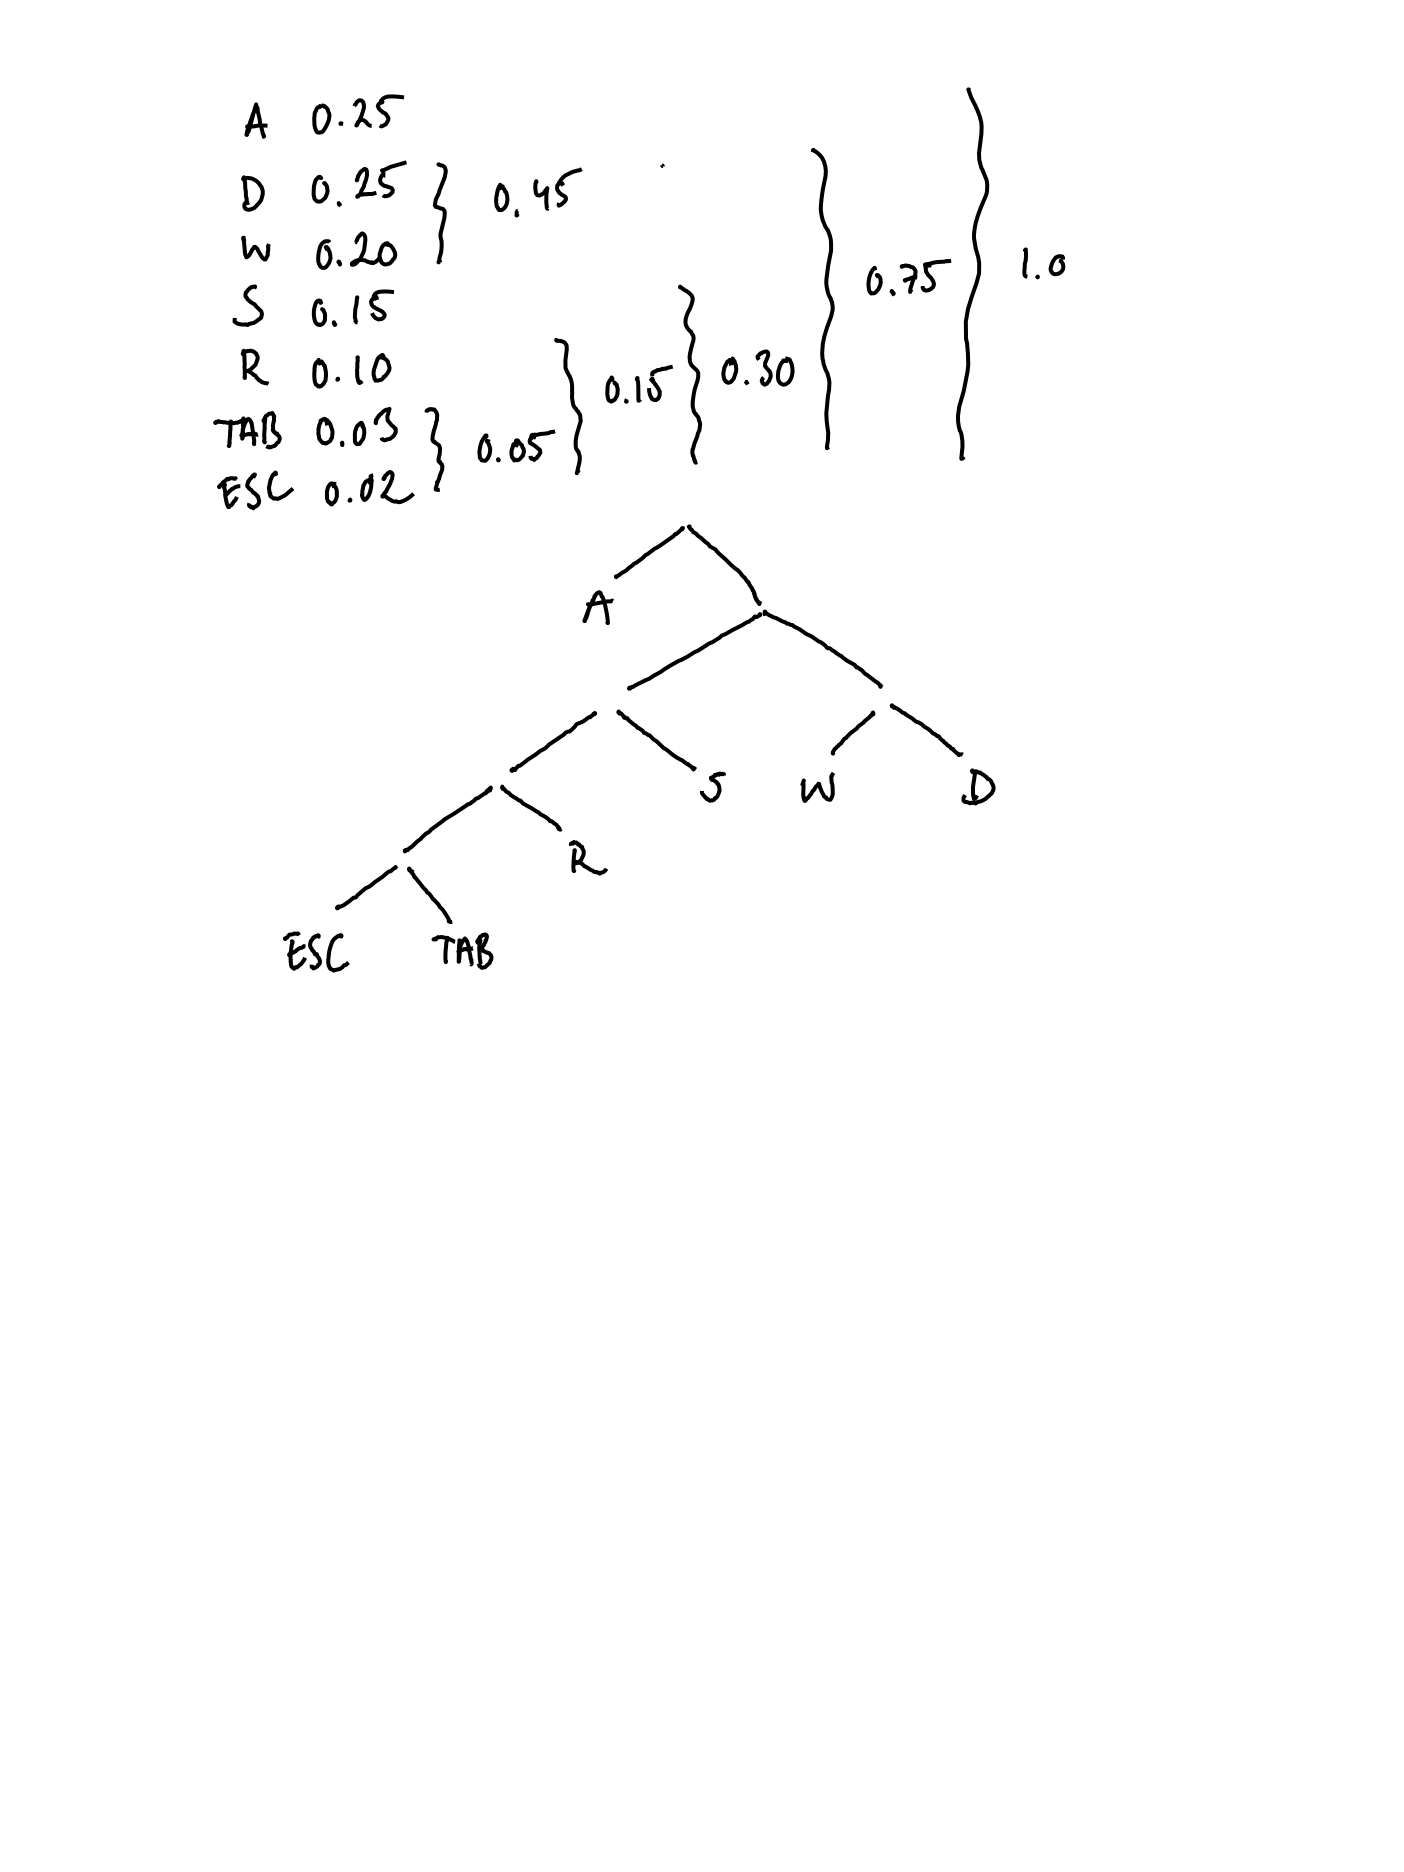
\includegraphics[height=0.8\textheight]{fig/overwatch-tree.pdf}
\end{frame}

\subsection{Mer huffmankodning}

\begin{frame}
  \begin{exercise}
    \begin{itemize}
      \item I Rövarspråket är \enquote{o}  mycket vanligare än alla andra 
        bokstäver.
      \item (Varje konsonantdubbleras, med o emellan, t ex skulle ”abc” bli 
        ”abobcoc” på rövarspråket.)
      \item Fyra av rövarna (Agata, Bobo, Cecil och Dorste) har beräknat 
        Huffmankoder förden givna frekvenstabellen, men alla har fått olika 
        svar.
    \end{itemize}
    \begin{enumerate}
      \item Vem har rätt? Avgör genom att rita huffmanträdet.
    \end{enumerate}
  \end{exercise}
\end{frame}

\begin{frame}
  \begin{table}
    \begin{tabular}{rrrrrr}
      \textbf{Bokstav} & \textbf{Frekvens}
          & \textbf{Agata} & \textbf{Bobo} & \textbf{Cecil} & \textbf{Dorste}
          \\
      O & 0.30 & 11 & 00 & 01 & 00 \\
      B & 0.16 & 10 & 10 & 110  & 010 \\
      D & 0.14 & 01 & 010 & 101 & 0110 \\
      N & 0.14 & 00 & 011 & 010 & 01110 \\
      T & 0.13 & 111 & 110 & 011 & 011110 \\
      A & 0.07 & 110 & 1110 & 1000 & 0111110 \\
      I & 0.06 & 101 & 1111 & 1100 & 0111111
    \end{tabular}
    \caption{Frekvenser och förslag på kodning.}
  \end{table}

  \begin{exercise}
    \begin{enumerate}
      \item Rita huffmanträdet och avgör vem som har kodat korrekt.
    \end{enumerate}
  \end{exercise}
\end{frame}

\begin{frame}
  \centering
  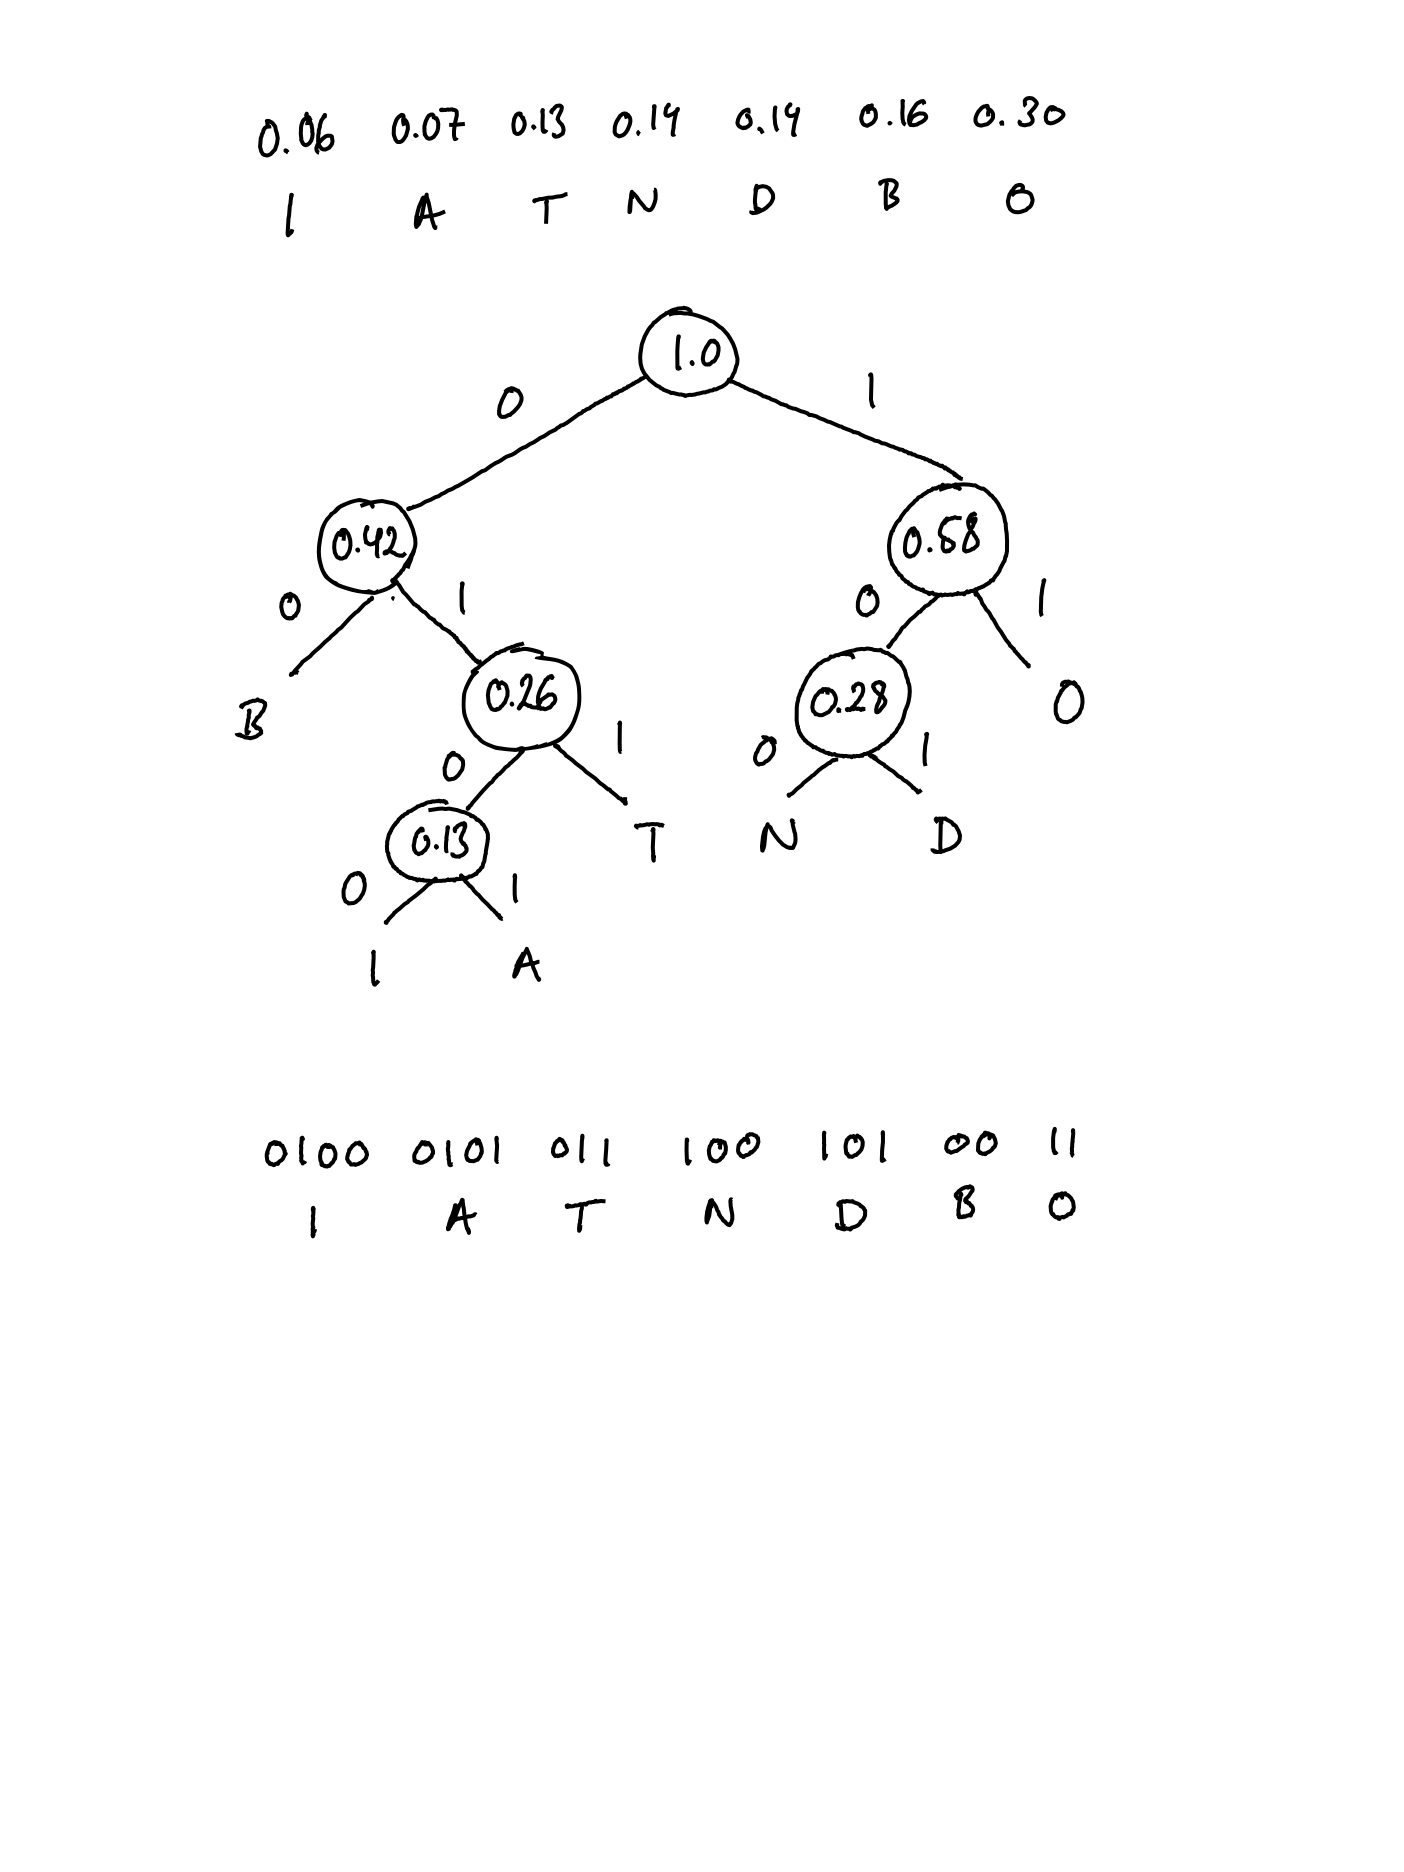
\includegraphics[height=0.8\textheight]{fig/rovar-tree-codewords.pdf}
\end{frame}

\section{Komprimera tentor}

\begin{frame}
  \begin{exercise}
    \begin{itemize}
      \item Dagen efter tentatillfället ska alla tentor scannas.
    \end{itemize}
    \begin{enumerate}
      \item Föreslå en komprimeringsmetodsom skulle kunna användas för 
        komprimering av den scannade tentan.
    \end{enumerate}
  \end{exercise}
\end{frame}

\begin{frame}
  \begin{solution}
    \begin{itemize}
      \item Förstörande metod funkar om handskriven inskanning.
      \item Digital tenta med text, icke-förstörande; exempelvis, Lempel-Ziv 
        eller Huffman.
    \end{itemize}
  \end{solution}
\end{frame}

\section{Redundans}

\begin{frame}
  \begin{columns}
    \begin{column}{0.7\columnwidth}
      \begin{exercise}
        \begin{itemize}
          \item Alla tecken som används i våra operativsystem använder någon 
            form av tecken-kodning.
          \item Den enklaste av dessa är ASCII med totalt 128 tecken.
          \item Det är en 7-bitars kod där varje tecken motsvarar ett visst 
            tal.
        \end{itemize}
        \begin{enumerate}
          \item Vad är minsta hammingavståndet för de binära koderna i hela 
            ASCII-tabellen?
          \item Hur skulle man kunna göra ASCII-koden mindre känslig för fel 
            vid överföring?
        \end{enumerate}
      \end{exercise}
    \end{column}
    \begin{column}{0.3\columnwidth}
      \begin{table}
        \begin{tabular}{rrr}
          A & 65 & 1000001 \\
          B & 66 & 1000010 \\
          C & 67 & 1000011 \\
          \vdots & \vdots & \vdots \\
          a & 97 & 1100001 \\
          b & 98 & 1100010 \\
          c & 99 & 1100011 \\
          \vdots & \vdots & \vdots
        \end{tabular}
        \caption{Ett utdrag ur ASCII-tabellen.}
      \end{table}
    \end{column}
  \end{columns}
\end{frame}

%\subsection{Mer komprimering}
%
%\begin{frame}
%\end{frame}

\mode*

\begin{frame}[allowframebreaks]
  \printbibliography
\end{frame}
\end{document}
